\documentclass{article}

%%% This file is the preamble for the Pomona Linguistics LaTeX Paper Template, which is also used for the Quick Reference Guide. If you are brand new to writing with LaTeX, we suggest NOT messing with it, and just writing your paper using the Paper Template. If you are getting more comfortable in LaTeX and want to add packages and commands, this is where you do it (when using this template).

%For stacking text, used here in autosegmental diagrams
\usepackage{stackengine}

%To combine rows in tables
\usepackage{multirow}

%geometry helps manage margins, among other things.
\usepackage[margin=1in]{geometry}

%Gives some extra formatting options, e.g. underlining/strikeout
\usepackage{ulem}

%For putting links into papers, also helps make cross-references in the paper smart references
\usepackage[colorlinks = true,
            linkcolor = blue,
            urlcolor  = blue,
            citecolor = blue,
            anchorcolor = blue]{hyperref} %smarter cross-references, these options turn links blue

%Use package/command below to create a double-spaced document, if you want one. Uncomment BOTH the package and the command (\doublespacing) to create a doublespaced document, or leave them as is to have a single-spaced document.
%\usepackage{setspace}
%\doublespacing

%paragraph formatting
\usepackage[parfill]{parskip}
\setlength{\parskip}{5pt} %plus 1 minus 1}
\setlength{\parindent}{30pt}
\usepackage{titlesec}

%use for special OT tableaux symbols like bomb and sad face. must be loaded early on because it doesn't play well with some other packages
\usepackage{fourier-orns}

%Basic math symbols
\usepackage{pifont}
\usepackage{amssymb}

%%%Gives shortcuts for glossing. The use of this package is NOT explained in the Quick Reference Guide, but the documentation is on CTAN for those that are interested. MJKD finds it handy for glossing. (https://ctan.org/pkg/leipzig?lang=en)
\usepackage{leipzig}

%Tables
\usepackage{caption} %For table captions
\usepackage{booktabs} %helps format tables

%For citations and bibliography - as of 9.1.2019 we don't explain citations in this Quick Reference Guide, but Pedro Martin's tutorial does (see links in the Guide).
\usepackage{natbib}

%For OT-style tableaux
\usepackage{ot-tableau}

%Fonts
%\usepackage[no-math]{fontspec} %This allows you to enter (via an IPA kayboard) IPA fonts and other symbols directly into LaTeX. Requires a particular setyp, see below.
\usepackage{libertine} %A font that actually contains many IPA symbols. This is the font you see in the preview to the right.

%to use these fonts, be sure that your typesetting engine is set to "XeLaTeX." In Overleaf, go to the Menu link on the top left (by the Overleaf icon), and under Settings be sure that the Compiler is set to "XeLaTeX." If you accessed this document via the Overleaf Pomona Linguistics template, all of this was already done for you.

%The Pomona Linguistics Paper Template in Overleaf is already set up for this, but you may run into this problem if you start building your own documents.

%highlights text with \hl{text}
\usepackage{color, soul}

%Drawing Syntax Trees
\usepackage[linguistics]{forest}

%This specifies some formatting for the forest trees to make them nicer to look at
\forestset{
  nice nodes/.style={
    for tree={
      inner sep=0pt,
      fit=band,
    },
  },
  default preamble=nice nodes,
}

%% For numbered and glossed examples %%
\usepackage{gb4e}



%Changes the \maketitle command to be smaller and take up less space on a page.
\makeatletter
\def\@maketitle{   % custom maketitle
\noindent {\Large \bfseries \color{black} \@title}  \\ \hrule \noindent \@author \\ \@date
}

%The code below will draw a circle around a piece of text. This is very useful for drawing attention to a word in a data example. use the command \circled{text} where the argument (`text' here) is what you want to be circled. This is illustrated in the Quick Reference Guide and the Paper Template.

\usepackage{tikz}

\newcommand{\circled}[1]{\begin{tikzpicture}[baseline=(word.base)]
\node[draw, rounded corners, text height=8pt, text depth=2pt, inner sep=2pt, outer sep=0pt, use as bounding box] (word) {#1};
\end{tikzpicture}
}


%%%%%%%%%%%%%%%%%%%%%%%%%%%%%%%%%%%%%%%%%%%%%%%%%%%%%%%%%%%%
%%%%%%%%%%%%%%%%%%%%%%%%%%%%%%%%%%%%%%%%%%%%%%%%%%%%%%%%%%%%

% Useful Ling Shortcuts

\RequirePackage{leipzig}
%\RequirePackage{mathtools} % for \mathrlap

% % % Shortcuts  (borrowed from JZ, I'm still unsure exactly what xspace requires)
\RequirePackage{xspace}
\xspaceaddexceptions{]\}}

%This makes the \emptyset command be a nicer one
\let\oldemptyset\emptyset
\let\emptyset\varnothing
\newcommand{\nothing}{$\emptyset$}

%Not all of these are explained in the Quick Reference Guide, but they are here bc they are relevant to some of our students.
\newcommand{\1}{\rlap{$'$}\xspace}
\newcommand{\0}{\rlap{\textsuperscript{$ˆ{\circ}$}}\xspace}
\newcommand{\Lb}[1]{$\text{[}_{\text{#1}}$ } %A more convenient left bracket
\newcommand{\Rb}[1]{$\text{]}_{\text{#1}}$ } %A more convenient left bracket
\newcommand{\gap}{\underline{\hspace{1.2em}}}
\newcommand{\vP}{\emph{v}P}
\newcommand{\lilv}{\emph{v}}
\newcommand{\Abar}{A$'$-} %A more convenient A-bar notation
\newcommand{\ph}{$\varphi$\xspace} %A more convenient phi
\newcommand{\pro}{\emph{pro}\xspace}
\newcommand{\subs}[1]{\textsubscript{#1}} %A more convenient subscript
%\newcommand{\hd}{$^{\circ}$\xspace} %Symbol for printing head / degree symbol
\newcommand{\spells}{$\Longleftrightarrow$} %spellout arrow for morph spellout rules
\newcommand{\tr}[1]{\textit{t}\textsubscript{\textit{#1}}} %easy traces with subscript
\newcommand{\supers}[1]{\textsuperscript{#1}}

% Abbreviations for glossing, based on Leipzig
\newleipzig{hab}{hab}{habitual}
\newleipzig{rem}{rem}{remote}
\newleipzig{sm}{sm}{subject marker}
\newleipzig{t}{t}{tense}
\newleipzig{aa}{aa}{anti-agreement}
\newleipzig{pron}{pron}{pronoun}
\newleipzig{rec}{rec}{recent}
\newleipzig{om}{om}{object marker}
%\newleipzig{ipfv}{ipfv}{imperfective}
\newleipzig{asp}{asp}{aspect}
\newleipzig{lk}{lk}{linker}
\newleipzig{pcl}{pcl}{particle}
\newleipzig{stat}{stat}{stative}
\newleipzig{ints}{ints}{intensive}
\newleipzig{ascl}{ascl}{assertive subject clitic}
\newleipzig{nascl}{nascl}{non-assertive subject clitic}
\newleipzig{ta}{ta}{tense and/or aspect}
\newleipzig{assoc}{assoc}{associative marker}
\newleipzig{hon}{hon}{honorific}
%\newleipzig{whprt}{wh}{\wh particle}
\newleipzig{sa}{sa}{subject agreement}
\newleipzig{conj}{conj}{conjunction}
%\newleipzig{loc}{loc}{locative}
\newleipzig{expl}{expl}{expletive}
\newleipzig{rcm}{rcm}{reciprocal marker}
\newleipzig{pers}{pers}{persistive}
%\newleipzig{}{}{} %this is just to copy for when I want to add more

%%%%%%%%%%%%%%%%%%%%%%%%%%%%%%%%%%%%%%%%%%%%%%%%%%%%%%%%%%%%
%%%%%%%%%%%%%%%%%%%%%%%%%%%%%%%%%%%%%%%%%%%%%%%%%%%%%%%%%%%%

%A couple of packages that seemed to prefer being called toward the end of the preamble

%This package provides macros for typesetting SPE-style phonological rules.
\usepackage{phonrule}

%For using Greek letters outside of math mode.
%\usepackage{textgreek}


%Random, lets us use the XeLaTeX logo. Not important to the template at all.
\usepackage{metalogo}


%%%%%%%%%%%%
%% This is the end of the PREAMBLE
%%%%%%%%%%%


\title{Tariana Paper 1}
\author{Skylar Litz}
\date{February 22, 2021}

\setlength\parindent{12pt}
%\hspace{\parindent} to get a tab

\begin{document}

\maketitle
\\
%\textbf{Research period 1:} word order of clauses and noun phrases, as well as other major features necessary to understand the basics of the language (e.g. basic morphology on nouns and verbs)
%\begin{abstract} Add abstract here?????
%\end{abstract}

\noindent All data, examples, and generalizations presented here come from \textit{A Grammar of Tariana, from Northwest Amazonia} by Alexandra Y. Aikhenvald (2003).

\section{Introduction}
\subsection{Background of Tariana}
  Tariana is an Arawak language spoken in the Vaupés basin in northwestern Brazil. In the past, Tariana was a ``dialect continuum'' spoken by over 1500 people living in settlements along the Vaupés river. The different subdialects of Tariana were about as different as the Romance languages are and constituted a strict hierarchy. When Catholic missions began to expand into the region, the groups that spoke the dialects of Tariana in the upper hierarchy abandoned the language and switched to Tucano. Now, the language is spoken by around 100 adults and all of them speak the previously lowest-ranking dialect, Wamiaɾikune.

	The Vaupés basin area is a multilingual area. All languages spoken in the area (besides Tariana) belong to the East Tucano subgroup of the Tucano family. There is a principle of linguistic exogamy in the region, meaning that you must marry someone who speaks a different language than you. Though this may imply lots of mixing between Tariana and local languages, there is a strong cultural inhibition against language mixing. Over time Tariana has inherited a few features from Proto-Arawak and East Tucano, though much of the language remains unique.

	% could also add more here such as bottom of pg 8 (31)

% chapter 3
\section{Word Classes}
Tariana has three open word classes, two semi-closed classes, and twelve closed classes.
\subsection{Open word classes}
The three open word classes in Tariana are verbs, nouns, and adjectives. Verbs are prototypical predicates, nouns are prototypical heads of noun phrases, and adjectives are prototypical modifiers.
\subsubsection{Verbs}
% nice summary of all verb things on pdf pg 89, maybe add in later?
Verbs can be divided into two categories, those which take prefixes and those which do not. Active verbs must take a cross-referencing prefix to mark the subject constituent. Stative verbs and verbs of physical state do not take any cross-referencing markers.
% there's some stuff here about obligatory prefixal positions and redicate-argument agreement/lack of it (pdf 89)

Tariana has ambitransitive verbs, meaning that some verbs can be either transitive or intransitive. In fact, every transitive verb in Tariana can be used in intransitive clauses. Most verbs are agentive ambitransitive verbs which means that the object NP can be omitted if desired. The example in Figure \ref*{eatpepper} shows an ambitransitive verb, where the object NP of `pepper' is optional in the phrase.

\begin{figure}[h!]
\centering
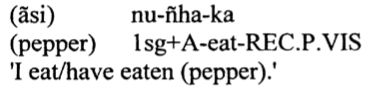
\includegraphics[scale = 0.38]{eatpepper.png}
	\caption{(Aikhenvald 2003 page 67)}
	\label{eatpepper}
\end{figure}
% there's some info on intransitive verbs, active verbs, stative verbs, verbs of physical state (pdf 90)

\subsubsection{Nouns}
Nouns in Tariana have grammatical categories of gender, noun classification, possession, number, case, nominal tense, and extralocality.

Nouns usually bear no gender marking, instead gender is expressed in person-number cross-referencing on verbs and obligatorily possessed nouns. Noun classification is shown through classifier agreement on modifiers in head-modifier NPs. Nouns can be divided into inalienably possessed (prefixed) and alienably possessed (prefixless). Number distinctions on nouns include singular, plural, unmarked, and associative. Nouns have three-fold tense distinction (past, future, and unmarked) and they can also be characterized for extralocality (if the participant referred to is in a different place or is not the one to do something).

% bruh so much of this is not very interesting.... maybe come back to it? (pdf 91)
The only nouns that can take a prefix are obligatorily possessed nouns which must take a possessive prefix. There is a closed subset of nouns called kinship nouns which must have a human (or animal) referent. There is also a closed class of `names of blessing' containing eleven members. These names are used very rarely, only on special occasions.

Vocative forms of personal names can be created by omitting the final syllable of a name and shifting the stress onto the last remaining syllable. For example, the vocative form of \textit{Olívia} is \textit{Olí}. Vocative forms of nouns with a human referent can be created in the same way. For example, in Figure \ref*{masterof} a vocative form \textit{miná} of \textit{mínaɾi} meaning `master of' is used.

\begin{figure}[h!]
\centering
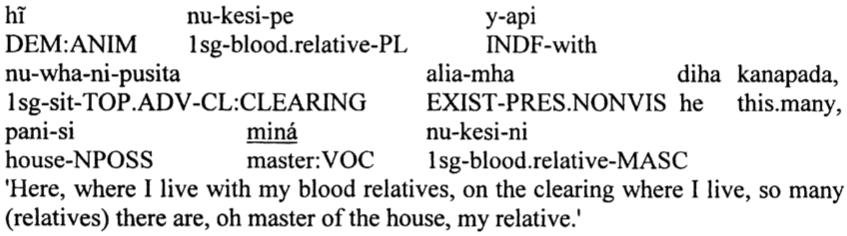
\includegraphics[scale = 0.38]{masterof.png}
	\caption{(Aikhenvald 2003 page 71)}
	\label{masterof}
\end{figure}

\subsubsection{Adjectives}
Any adjective in Tariana can be used without a nominal head in a noun phrase. For example, \textit{inaɾu matʃi:te} means `bad woman' while \textit{matʃi:te} just means `bad one.' Adjectives can be underived or derived. Underived adjectives form a class of around twenty items. There are no specific adjectives that refer to form (such as `round' or `hollow'), instead those meanings can be conveyed using classifiers.

The underived adjectives can be split into semantic groups of dimension, age, value, color, and physical properties. There is one further adjective that does not belong to any of those semantic groups which is \textit{keninite} meaning `loved (by women).' This adjective is not used very frequently.

All adjectives require classifier agreement with the head noun. For adjectives with an inanimate referent, number agreement is optional. For human and higher animates, number agreement is required. Adjectives have most nominal grammatical categories, except an adjective cannot have a tense or extralocality value that is different from the head noun. The example in Figure \ref*{bigtree} illustrates classifier agreement with an underived adjective, \textit{hanu}. In Figure \ref*{eyelessman}, classifier agreement on an adjective derived from a verbal phrase is shown.

\begin{figure}[h!]
\centering
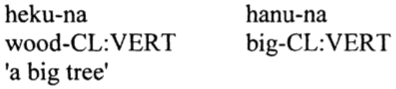
\includegraphics[scale = 0.38]{bigtree.png}
	\caption{(Aikhenvald 2003 page 73)}
	\label{bigtree}
\end{figure}

\begin{figure}[h!]
\centering
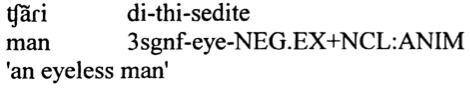
\includegraphics[scale = 0.38]{eyelessman.png}
	\caption{(Aikhenvald 2003 page 74)}
	\label{eyelessman}
\end{figure}

% maybe add stuff about suffix/clitic -iha which behaves interestingly (pdf 97)

\noindent Adjectives share the following properties with nouns:
\begin{enumerate}
  \item They can be used as NP heads without special word class-changing morphology
  \item They can be used as copula complements %(see \ref*{Copula})
\end{enumerate}

\noindent Adjectives share the following properties with stative verbs:
\begin{enumerate}
  \item When used as predicates they take the same morphology as stative verbs
  \item They can be used in some imperative clauses similarly to stative verbs
  \item Underived adjectives can never take cross-referencing prefixes
\end{enumerate}

\noindent Finally, there are some properties which are unique to adjectives (not shared with nouns or verbs). These include:
\begin{enumerate}
  \item Classifiers of all types are used as agreement markers with adjectives
  \item Plurality is an agreement category for adjectives (unlike nouns) but adjectives do not have some of the plural forms that nouns have
  % the rest are mostly about -iha, see pdf pg 99
\end{enumerate}

% pdf pg 100
%\subsection{Word Class-Changing Morphological Derivations}

\subsection{Semi-Closed Classes}
\subsubsection{Manner Adverbs}
Most manner adverbs in Tariana arise from a reinterpretation of serial verb constructions. Adverbs cannot take case marking, their function is to modify a verb or a predicate. The roots of underived adjectives can be used as value adverbs. Figure \ref*{raining} illustrates the simple adverb \textit{some} meaning 'a lot'.

\begin{figure}[h!]
\centering
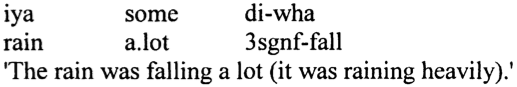
\includegraphics[scale = 0.38]{raining.png}
	\caption{(Aikhenvald 2003 page 78)}
	\label{raining}
\end{figure}

\subsubsection{Time Words} \label{Time Words}
Unlike manner adverbs, time words can take the non-subject case enclitic \textit{-nuku} when they are typical. They can also take the locative case \textit{-se}. They cannot take any other noun morphology and cannot be used as arguments of verbs. Figure \ref*{poisonfish} shows \textit{desu} meaning 'tomorrow' when it is not topical, while \ref*{eattomorrow} shows \textit{desu} when it is topical, thus is marked with \textit{-nuku}.

\begin{figure}[h!]
\centering
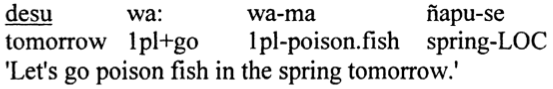
\includegraphics[scale = 0.38]{poisonfish.png}
	\caption{(Aikhenvald 2003 page 79)}
	\label{poisonfish}
\end{figure}

\begin{figure}[h!]
\centering
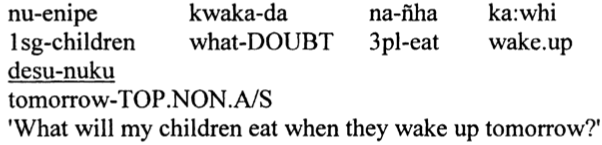
\includegraphics[scale = 0.38]{eattomorrow.png}
	\caption{(Aikhenvald 2003 page 79)}
	\label{eattomorrow}
\end{figure}

\subsection{Closed Classes} \label{Closed Classes}
The closed word classes that can be used as NP heads and as modifiers are personal pronouns, specifier articles, interrogative-distributive \textit{kwa/kwe}, demonstratives, gestural deictic \textit{khi}, distributive individualizer \textit{napada}, general indefinite \textit{pa-}, numerals, and quantifiers. Adpositions are also a closed word class and can only be used as NP heads.

\subsection{Overview of Word Classes}
Figure \ref*{wordclasstable} summarizes the relationships between major word classes and functional slots.

\begin{figure}[h!]
\centering
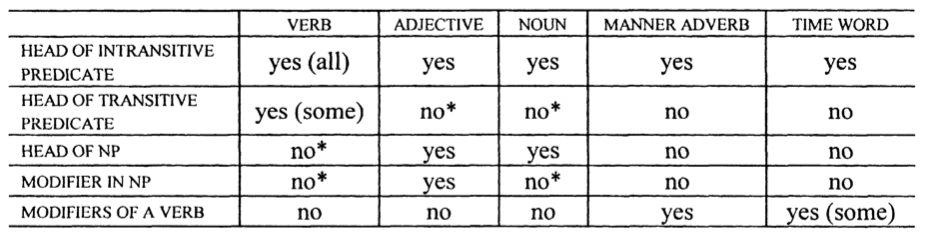
\includegraphics[scale = 0.45]{wordclasstable.png}
	\caption{(Aikhenvald 2003 page 81)}
	\label{wordclasstable}
\end{figure}

% chapter 4: pg 475 (pdf 498)
%\section{Nominal Morphology and Noun Structure}

% chapter 21
\section{Clause Types}
Independent clauses can be declarative, imperative, interrogative, and exclamatory. The different types differ in their ability to express verbal categories, especially tense-evidentiality.

\subsection{Declarative Clauses} \label{Declarative Clauses}
Declarative clauses have variable constituent order and their predicate has the full set of tense-evidentiality distinctions. % add reference here to tense-evidentiality?

% pdf pg 511
\subsubsection{Copula Clauses} \label{Copula}
% there are SO MANY TYPES OF COPULA ??!!!?!!?
Copula clauses can express existence, location, and possession; identity and equation; physical and mental state; becoming; similarity and appearance; and naming. Though different types of copula clauses employ different copula verbs and have different structures, the range of copulas covered by this paper is limited. % maybe change this in the future...?

The prefixless copulas \textit{alia} and \textit{sede} can appear with one argument which usually indicates existence. An example of this is shown in Figure \ref*{dancemaster} where the copula clause is in brackets and the copula is underlined.

\begin{figure}[h!]
\centering
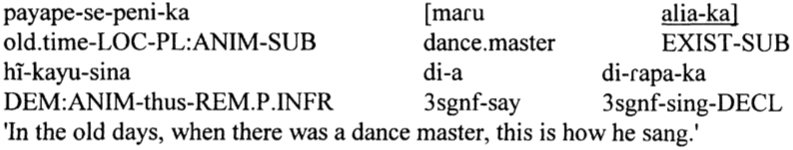
\includegraphics[scale = 0.4]{dancemaster.png}
	\caption{(Aikhenvald 2003 page 488)}
	\label{dancemaster}
\end{figure}

% pdf pg 520
\subsubsection{Verbless Clauses}
Verbless clauses are used to express existence, location, identity and equation, mental and physical state, as well as attribution and evaluation. Some of these clauses are allowed to also contain a copula, in which case there is a difference in meaning. Verbless existential clauses only appear at the beginning of narratives to introduce participants. Verbless locational clauses are frequent and can be used anywhere as long as the location is clear from context. In identity and equation clauses which are verbless, the copula is only used if the copula complement is focussed or unexpected. An example of this is provided in Figure \ref*{schoolteacher} where the speaker is introducing a piece of focussed piece of information that he is the local school teacher.

\begin{figure}[h!]
\centering
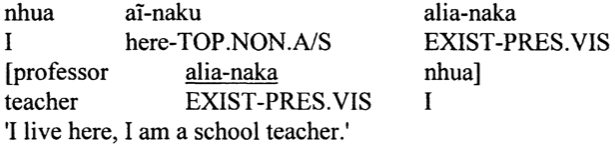
\includegraphics[scale = 0.4]{schoolteacher.png}
	\caption{(Aikhenvald 2003 page 498)}
	\label{schoolteacher}
\end{figure}

% pdf pg 523
\subsubsection{Intransitive Clauses}
Intransitive clauses can be divided into three types: strictly intransitive, double S-clauses, and extended intransitive. Strictly intransitive clauses contain an intransitive verb as their predicate and can contain obliques such as a beneficiary. An example of this is shown in Figure \ref*{legsaching}.

\begin{figure}[h!]
\centering
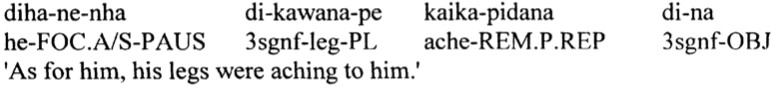
\includegraphics[scale = 0.4]{legsaching.png}
	\caption{(Aikhenvald 2003 page 500)}
	\label{legsaching}
\end{figure}

Double S-clauses are a subtype of intransitive clauses that refer to emotional states and contain an inalienably possessed body part preposed to the predicate. Extended transitive clauses contain prefixless verbs and two obligatory arguments, one of which is the subject, the other of which can take non-subject case-marking.

% pdf pg 524
\subsubsection{Transitive and Ditransitive Clauses}
Transitive and ditransitive clauses contain a transitive or a ditransitive verb as a predicate. All verbs of these types mark their non-subject arguments with the non-subject case. The constituent order in these clauses follows the descriptions provided in Section \ref*{Constituent Order}.

% pdf pg 525 - very short
\subsection{Imperative Clauses} \label{Imperative Clauses}
In imperative clauses, the predicate must contain a verb in an imperative form. These clauses have a higher pitch and a stronger intensity on the stressed syllable of the predicate.
% imperative clauses do not have evidentiality marking

% pdf pg 525
\subsection{Interrogative Clauses} \label{Interrogative Clauses}
Interrogative clauses have a different set of tense-evidentiality markers compared to declarative clauses. % add reference here
Content questions contain a question word while polar questions do not, instead they are distinguished by rising intonation and the choice of an evidential marker. Questioning more than one constituent is not allowed, nor is questioning constituents in subordinate clauses. It is not culturally appropriate to ask too many questions in Tariana as when a question is asked, it is often seen as the asker doubting the addressee.
% this is super interesting, more information to come when looking at tense-evidentiality!

% pdf pg 529
\subsection{Exclamatory Clauses} \label{Exclamatory Clauses}
Exclamatory clauses have no tense-evidentiality specifications and usually consist of one word, one NP, or just a predicate. They often have a slightly rising intonation and the stressed syllable is pronounced with more intensity. An example of this is seen in Figure \ref*{bigbaby} when the speaker reacts surprisedly to a large baby. In this example, the underlined vowel \emph{ú} is stressed.

\begin{figure}[h!]
\centering
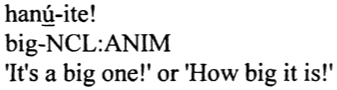
\includegraphics[scale = 0.4]{bigbaby.png}
	\caption{(Aikhenvald 2003 page 506)}
	\label{bigbaby}
\end{figure}

% there's some stuff after this about the different subject types, seems kind of interesting but not super important maybe?

\subsection{Structure of Noun Phrases}
A noun phrase consists of a head plus one or more modifiers. There is no basic order for NPs, the ordering is always pragmatically conditioned.
% NP Heads
NP heads can be a noun, adjective, or a member of one of the closed classes mentioned in Section \ref*{Closed Classes}. The head of an NP forces classifier (or animacy) agreement on any modifier that is present on the head. Animate NP heads also force number agreement.
%NP Modifiers
NP Modifiers can be adjectives, members of closed classes, and some nouns.

\subsubsection{Position of Modifiers in Noun Phrases}
 Adjectives or closed class modifiers can be used in either the prehead or posthead position, except for specifier articles, demonstratives, and the quantifier \textit{kanapada}, which always precede the NP head. The placement of modifiers prehead or posthead depends on the definiteness and specificity of the head noun. If a noun is definite or specific, modifiers tend to be placed before the noun. Indefinite or non-specific nouns usually have modifiers placed after the noun. For example (Figure \ref*{naughtytapir}), in a story being told about a well-known naughty tapir who destroys gardens, the modifier adjective `bad' is placed before the head noun, `tapir.'

\begin{figure}[h!]
  \centering
  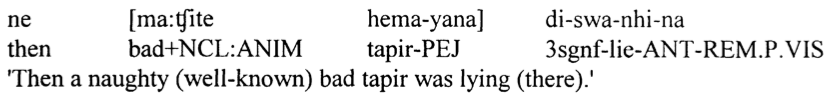
\includegraphics[scale = 0.4]{naughtytapir.png}
    \caption{(Aikhenvald 2003 page 476)}
    \label{naughtytapir}
\end{figure}

\noindent An NP can contain only one prehead modifier, so if one modifier is required to appear before the noun, the rest will appear after. For example, though demonstratives precede the head of an NP, if the prehead position contains an interrogative modifier in an interrogative clause, they will follow the head of the NP instead. In Figure \ref*{aracufish}, the noun phrase in brackets contains both a prehead and posthead modifier. The adjective 'bad' could not appear before the head in the NP because the prehead modifier slot is filled with the demonstrative.

\begin{figure}[h!]
  \centering
  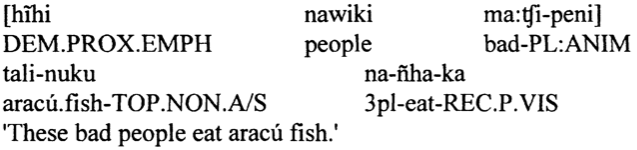
\includegraphics[scale = 0.39]{aracufish.png}
    \caption{(Aikhenvald 2003 page 479)}
    \label{aracufish}
\end{figure}

\subsubsection{Discontinuous Noun Phrases}
A split NP occurs when the head occurs before the predicate and the modifiers occur after it or when the head occurs after the predicate and the modifiers occur before. Afterthoughts and discontinuous NPs are distinguished by the presence or lack of a pause before the modifier. If there is a pause, it is an afterthought. If there is no pause, it is a discontinuous NP. One use of split NPs is to introduce a referent whose identity is supposed to be unknown to the speaker but is important. The example in Figure \ref*{lookingforwomen} is from a story of a man looking for women. Once he found one, he presented her to his mother saying the phrase in \ref*{lookingforwomen}.

\begin{figure}[h!]
  \centering
  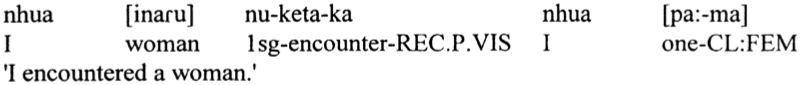
\includegraphics[scale = 0.4]{lookingforwomen.png}
    \caption{(Aikhenvald 2003 page 480)}
    \label{lookingforwomen}
\end{figure}

\subsubsection{Appositional Constructions}
Appositional constructions consist of a noun modifying another noun. Nouns which can modify other nouns are proper names, kinship terms, and generic nouns. Proper nouns and kinship terms follow the head noun and there is no pause between the head noun and the modifier. The generic noun \textit{yaphini} meaning 'thing' occurs before the noun it modifies when it means '(what) kind of thing' such as in Figure \ref*{whatanimal}.

\begin{figure}[h!]
  \centering
  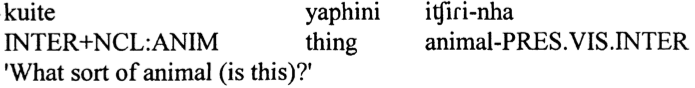
\includegraphics[scale = 0.4]{whatanimal.png}
    \caption{(Aikhenvald 2003 page 482)}
    \label{whatanimal}
\end{figure}

\noindent Only the time words (see \ref*{Time Words}) \textit{heku} meaning 'yesterday', \textit{ikasu} meaning 'today', and \textit{desu} meaing 'tomorrow' can occur in an appositional construction with another time word. For example, \textit{heku hekwa} meaning 'yesterday noon' is allowed.

\subsubsection{Headless Noun Phrases} \label{Headless NPs}
In narratives and conversations, full NPs are not very frequent. Instead, headless NPs are used in which a classifier is used to identify the referent. For example (Figure \ref*{oneman}), the man who lives alone with his children is introduced in a headless NP with a numeral and a classifier.

\begin{figure}[h!]
  \centering
  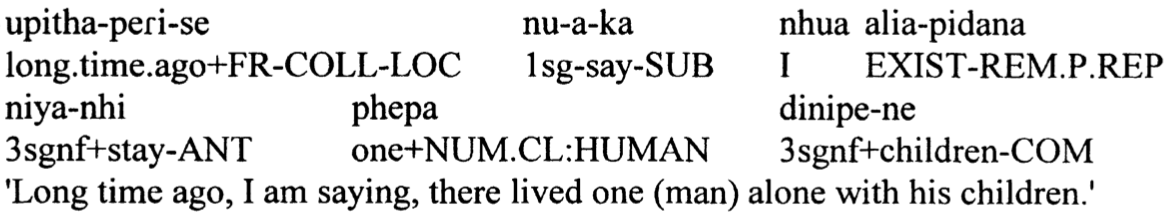
\includegraphics[scale = 0.49]{onemanexample.png}
    \caption{(Aikhenvald 2003 page 482)}
    \label{oneman}
\end{figure}

% \subsubsection{Possessive and Adpositional Noun Phrases}

% pg 585
%Some modifiers including demonstratives usually precede the head of the NP, only following it if the prehead position contains an interrogative modifier in an interrogative clause.
% Heavy modifiers, including relative clauses, are always posthead.

%[SEE CHAPTER 5] (more on this in second presentation? or add diarrhea example from page 93 (pdf pg 116))

% possessive constructions the possessor always precedes the possessed noun (different from different Arawak languages) pg 506

% chapter 25: pg 561 (pdf 584)
\section{Constituent Order} \label{Constituent Order}
Tariana is a \textit{pragmatically ordered} language so establishing a basic constituent order is not possible. In both texts and conversations, any constituent order is possible and all different organizations are used.

There are a few situations when Tariana may appear to have a fixed constituent order, or at least a prevalent constituent order. Sentences that are translated from the nearby language Tucano are generally \textit{verb-final} while sentences translated from Portuguese are often \textit{verb-medial}. For this reason, when studying Tariana it is important not to rely on translated material to understand constituent order. Aikhenvald notes that she followed this principle throughout the grammar, thus the data presented should be representative of how native speakers speak.

% pg 586 of pdf
Instead of having a set constituent order, pragmatic parameters are used to order constituents in main clauses. These parameters include new vs. old information, relative topicality, definiteness, specificity, and contrast.

\subsection{Pragmatic Parameters}
\subsubsection{Clause-Initial and Pre-Predicate Positions: Topicality} % pdf pg 586
A newly introduced or continuous topic that is a subject occupies the clause-initial position. If a subject that has just been introduced as a future topic of a narrative is present in the next clause, the subject will again occupy the clause-initial position. This can be seen in Figure \ref*{jaguar1} and \ref*{jaguar2}. In \ref*{jaguar1}, a jaguar is introduced as the subject at the beginning of the clause. Then, in the following sentence in Figure \ref*{jaguar2}, the same jaguar is mentioned again at the beginning of the clause as well, this time with the specifier article ``diha.''

\begin{figure}[h!]
  \centering
  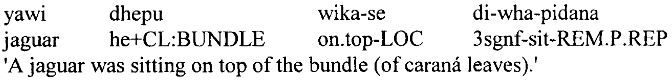
\includegraphics[scale = 0.44]{jaguar1.png}
    \caption{(Aikhenvald 2003 page 205)}
    \label{jaguar1}
\end{figure}

\begin{figure}[h!]
  \centering
  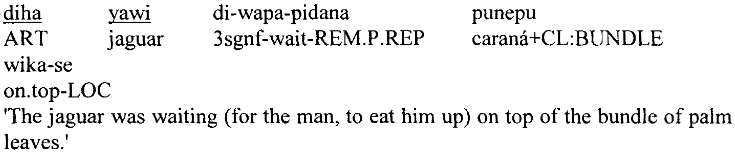
\includegraphics[scale = 0.44]{jaguar2.png}
    \caption{(Aikhenvald 2003 page 205)}
    \label{jaguar2}
\end{figure}

\noindent If a new topic is unexpected and important, it can be marked with the focussed A/S case \textit{-nhe/-ne}. % more info 7.2.1, 7.5a, 25.2a

\noindent Any constituent that is more topical than the subject of a clause can occupy the clause-initial position. In Figure \ref*{thistell}, 'this' refers to the content of the story, the topic of the preceeding conversation.

\begin{figure}[h!]
  \centering
  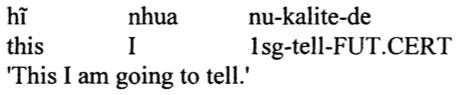
\includegraphics[scale = 0.38]{thistell.png}
    \caption{(Aikhenvald 2003 page 563)}
    \label{thistell}
\end{figure}

\noindent Normally, the A/S and O constituents are omitted once they have been introduced as they are clear from context. However these constituents can be repeated to create a comic effect, as if 'overstating' the situation.

\noindent There is also a specific case marking, \textit{-nuku}, for topical non-subjects.
% maybe add stuff about what happens if there are more than one -nuku in a sentence? pdf pg 588
\subsubsection{Post-Predicate Positions: Contrast and/or Disambiguation}
The post-predicate position is filled by contrastive or unexpected participants. If the subject constituent is placed in this position in an introductory clause, it creates unexpectedness. For example, in Figure \ref*{oneman}, a man who lives with his children is a subject that occupies the postpredicate position. The man is unexpected as a man living with his children is rare in Vaupés society. A postponed subject like in this example is usually separated from the predicate by a short pause.

The \textit{-nhe/-ne} case discussed earlier can be used on an A/S constituent after the predicate if it is strongly contrastive. Generally constituents marked with the contrastive \textit{-se} are preposed to the predicate if topical, but can occupy the post-predicate position if they are an unexpected participant. For example, in Figure \ref*{unexpectedwoman}, a man looks at a woman who is unexpected and the constituent of the woman with the \textit{-se} marker is in the post-predicate position.

\begin{figure}[h!]
  \centering
  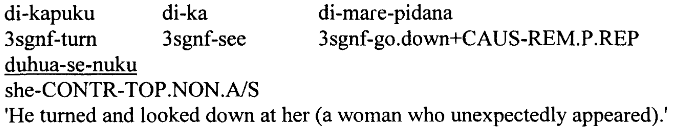
\includegraphics[scale = 0.43]{unexpectedwoman.png}
    \caption{(Aikhenvald 2003 page 191)}
    \label{unexpectedwoman}
\end{figure}

Verb-initial clauses followed by two NPs (either VAO or VOA) are rare and only occur if both A and O are contrastive. In this case, the constituent that is the most contrastive, or is used for clarification, occupies the clause-final position. Either A, O, or both must be marked with the topical non-subject marker \textit{-nuku} or the focussed A/S marker \textit{-nhe/-ne}.

Constituents which are used as afterthoughts or as clarifications also appear in the post-predicate position and are signaled by a preceding phrase-final falling intonation. Any constituent can be an afterthought.

\subsubsection{Unmarked Non-Subject Immediately Before the Predicate}
The only time an indefinite and non-specific non-subject noun unmarked for the \textit{-nuku} case is places immediately before the verb is when the whole construction is used to describe an activity. For example, Figure \ref*{fishing} describes a man going fishing.

\begin{figure}[h!]
  \centering
  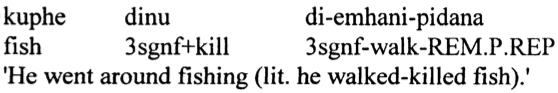
\includegraphics[scale = 0.4]{fishing.png}
    \caption{(Aikhenvald 2003 page 567)}
    \label{fishing}
\end{figure}

% pdf pg 591
\subsection{Constructions with Fixed Constituent Order}
There are only a few cases when strict ordering principles apply in Tariana. These are, % maybe add more examples here?

\begin{enumerate}
  \item \textbf{Position of the Copula Complement.}\\
  Copula components were discussed in \ref*{Copula}.
  The copula itself can generally only be clause-final or clause-medial, but the existential copula can be clause-initial. The copula complement cannot be separated from the copula \textit{alia} in identity and equation classes. A copula complement used to describe physical and mental states can occupy the clause-initial topical position and allow another constituent to intervene between the complement and the copula. An example of this can be seen in Figure \ref*{hungerexisted}.

  \begin{figure}[h!]
    \centering
    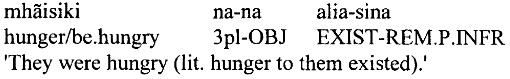
\includegraphics[scale = 0.42]{hungerexisted.png}
      \caption{(Aikhenvald 2003 page 492)}
      \label{hungerexisted}
  \end{figure}

  \item \textbf{Position of Interrogative Words} \\
  Interrogative words occupy the initial position in a content question. When used in relative clauses or complement clauses they also tend to occupy the clause-initial position. When the subject is expressed with an overt NP, the preferential order is Interrogative-Predicate-A/S. A topical constituent can be preposed to the interrogative, as in Figure \ref*{mysongone} where the subject \textit{nuɾi} comes before the interrogative word \textit{kani}.

  \begin{figure}[h!]
    \centering
    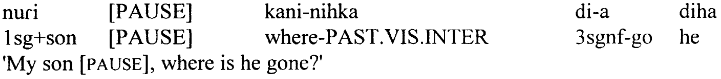
\includegraphics[scale = 0.45]{mysongone.png}
      \caption{(Aikhenvald 2003 page 313)}
      \label{mysongone}
  \end{figure}

  \item \textbf{Position of Connectors} \\
  Clause and sentence connectors occupy the sentence-initial position. Examples of connectors include \textit{diwese, diwesew(h)ya} meaning 'then', \textit{kayumaka} meaning 'so, thus', and \textit{kay di-ni} meaning 'so he did'.

  \item \textbf{Position of the Predicate of Dependent Clauses} \\
  Dependent clauses and nominalizations exhibit strictly predicate-final constituent ordering. The only exception to this is the discourse-organizing phrase \textit{nu-a-ka nhua} (1sg-say-\textsc{sub} I) meaning 'I am saying' or 'as I am saying.' This phrase is extremely common in narratives of all genres.

  \item \textbf{Subjects of Imperatives and Apprehensives} \\
  If the subject of an imperative is stated, it follows the predicate. One exception is when a subject of a detrimental imperative is highly topical, in which case the subject can precede the predicate.

  \item \textbf{Double S-clauses} \\
  Double S-clauses always follow the order of body part followed by predicate.
\end{enumerate}

% doubling of personal pronouns (pdf 594)

\subsection{Ellipsis} \label{Ellipsis}
Narratives and conversations in Tariana are highly elliptic. This means that participants are often left unspecified and must be identified using cross-referencing, classifiers, and context (see \ref*{Headless NPs}). In Figure \ref*{twoducks}, a man meets two ducks and the NP meaning 'they' is omitted.

\begin{figure}[h!]
  \centering
  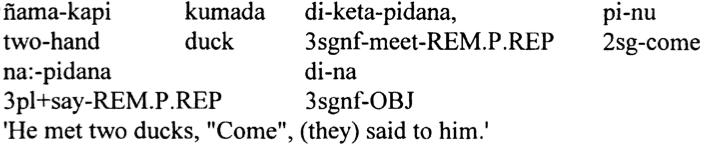
\includegraphics[scale = 0.39]{twoducks.png}
    \caption{(Aikhenvald 2003 page 573)}
    \label{twoducks}
\end{figure}

\noindent In Figure \ref*{strengthleft}, it is clear from context that strength is missing, so the NP for strength is omitted.

\begin{figure}[h!]
  \centering
  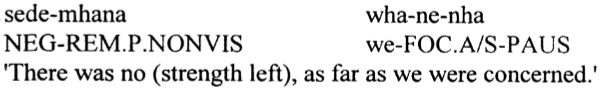
\includegraphics[scale = 0.42]{strengthleft.png}
    \caption{(Aikhenvald 2003 page 573)}
    \label{strengthleft}
\end{figure}

\noindent Due to ellipsis as well as cross-referencing on transitive and active intransitive verbs, only around 10 per cent of transitive clauses in Tariana have two NPs.

%\subsection{Repetition} \label{Repetition}
% some other things in here
% grammatical properties of narratives and conversations (pdf 608) this is interesting, not sure if worth mentioning here though

\end{document}
